\chapter{Methodology}
\label{sec:method}

The research questions contain three main points, outlining the methodology of the study: exploring the relationship between select road network attributes and adjacent \gls{lulc} classes, integrating them into the feature space of the \gls{lulcu} with a suitable encoding method, and in the end evaluating its impact regarding the model's performance. The assessment of the relationship between roads and adjacent \gls{lulc} classes includes preprocessing the road network and following a methodology which spatially joins the road network to the \gls{lulc} classes. Based on this spatial join, the relationship can be analyzed statistically. The findings are used for the development of multiple methods for feature engineering and encoding the road network, facilitating its integration into the feature space of the \gls{lulcu}. The last step is to evaluate the impact of the road network as spatial contextual information on the model's performance and resource consumption, which is done by comparing the baseline model to different so called extensions with differently encoded road network attributes integrated into the feature space of the model.

%%%%%%%%%
\section{Study Area}

The selected study area is located in Baden-Württemberg in the southwest of Germany and spans an area of approximately 1,314 km². The area is composed of the home town of the university this thesis is written at, the city of Heidelberg, along with two adjacent areas, the city of Mannheim and the Rhein-Neckar-Kreis, all part of the Rhine-Neckar Metropolitan Region.

Heidelberg is a city with approximately 160,000 inhabitants on an area of about 109 km², known for its picturesque old town, the Heidelberg Castle, and the oldest university in Germany, the Ruprecht-Karls-Universität Heidelberg \autocite{Heidelberg2024a}. Its landscape is characterized by a mix of urban areas and farmlands, with the Neckar river running through the city and the Odenwald, a low mountain range with large areas covered by forests, making a large part of the city's area in the east \autocite{Heidelberg2024b}.

Mannheim is the second largest city of Baden-Württemberg, spanning roughly 145 km² with nearly 312,000 inhabitants further northwest of Heidelberg, known for its grid-like city layout and the Palace of Mannheim. Due to its size and location at the confluence of the rivers Rhine and Neckar, it is an important economic hub in the region. Its landscape is more urban than Heidelberg's \autocite{Mannheim2024}. The Rhein-Neckar-Kreis almost surrounds the city of Heidelberg completely, the city of Mannheim only borders Heidelberg to the northwest.

Spanning an expansive area of about 1,061 km² and home to over 556,000 people, the Rhein-Neckar-Kreis is by far the largest of the three areas. This rural district is renowned for its vineyards, the Neckar river, and the Odenwald. It primarily consists of farmlands, forests, and many spatially distributed small towns and cities across the area \autocite{Rhine-Neckar2024,Rhein-Neckar-Kreis2024}. Figure \ref{fig:mahdrnk} shows the selected area of interest with \gls{lulc} classes provided by \gls{osm}Landuse \autocite{Schultz.Voss.ea2017}.

\begin{figure}[htb]
    \centering
    \includegraphics[width=\textwidth]{Figures/maps/MAHDRNK.pdf}
    \caption[Overview over the \glsentrylong{aoi} \glsfmtshort{mahdrnk}]{Selected \gls{aoi}, composed of the cities of Mannheim and Heidelberg as well as the adjacent Rhein-Neckar-Kreis in southwest Germany. The colors represent the land use and land cover classes, provided by \gls{osm}Landuse, and the boxes represent the patches calculated by the area descriptor module of the \gls{lulcu}.}
    \label{fig:mahdrnk}
\end{figure}

The \gls{aoi}, called \gls{mahdrnk} from this point on, is located in the northwest of Baden-Württemberg, blending the parts of the Odenwald low mountain range and the Upper Rhine Rift Valley. Incorporating two larger and many smaller cities as well as large rural regions, it is characterized by a heterogeneous \gls{lulc} composition. As seen in figure \ref{fig:mahdrnk}, this includes urban and rural areas, water bodies, forests, different artificial land uses, as well as large farmland patches. Moreover, it features a diverse relief, a result of the geographical influences of the rift valley and the Odenwald, all within a comparatively small area.

The area descriptor module of the \gls{lulcu}, explained further below, splits the \gls{aoi} in 19 rectangular patches. These can also be seen in figure \ref{fig:mahdrnk}. 

%%%%%%%%%%
\section{Data}

This section describes the various datasets utilized for the explorative relationship analysis and model training, including \gls{osm}, road networks and \gls{lulc} classes from \gls{osm}, as well as satellite imagery. All datasets, except those automatically created during model training, are queried for the timestamp \emph{2024-03-15T 00:00:00Z} to ensure consistency and comparability.

%%%%%%%%%%
\subsection{\glsentrylong{osm}}
\label{subsec:osm}

The \gls{lulcu} utilizes \gls{osm} data as ground truth (true) labels for the \gls{lulcm}. That is because studies have shown its suitability for remote sensing based \gls{lulcm} \autocite{Usmani.Napolitano.ea2023,Yang.Fu.ea2017}. \textcite{Schott.Zell.ea2024}, furthermore, evaluated the suitability of \gls{osm} for deriving \gls{lulc} labels for remote sensing-based models. They based their analysis on intrinsic quality indicators of the data and concluded that using \gls{osm} proves high potential for \gls{lulcm}.

\gls{osm} is the world's largest community-based Volunteered Geographic Information mapping project. It provides free geographical vector data of different scale, including buildings, roads, borders, as well as other geographical features. The database is publicly accessible and maintained by a global community of volunteers. The community comprises both individual contributors as well as organized mapping communities, including corporate and humanitarian organizations, which contribute to \gls{osm} collectively through organized mapathons \autocite{Anderson.Sarkar.ea2019,Herfort.Lautenbach.ea2021}. These contributors gather data from a variety of sources, including manual digitization of ortho-rectified satellite imagery, GPS data collection, data imports from other databases, and local knowledge for data verification \autocite{Usmani.Napolitano.ea2023}.

%%%%%%%%%%
\subsubsection*{Data Structure}

A unique aspect of \gls{osm} is its use of a hierarchical data structure to organize object-related data. This data can be utilized to efficiently extract or filter information relevant to specific geographical applications or problems \autocite{Schott.Zell.ea2024}. \gls{osm} utilizes three main data elements: nodes, ways, and relations.

A node, defined by latitude and longitude, represents a specific point on Earth. Each node has an ID and coordinates. Nodes can depict standalone features like a tree or a a park bench, or define a way's shape. When part of ways, nodes usually lack tags, but exceptions exist, like traffic signals on roads or pylons on power lines. Nodes can also be members of relations, with their roles indicated within the relation \autocite{Minghini.Frassinelli2019,OSMWiki2024}.

A way is the second fundamental map element, representing linear features like roads or rivers. It is an ordered list of at least two nodes and can be open or closed. Closed ways, where the first and last node are the same, can depict area boundaries like buildings or forests. However, they can also represent loops, such as roundabouts. Tags on the way help distinguish between these uses. If a way consists of more than 2,000 nodes, a more complex MultiLineString or MultiPolygon relation data structure will be required instead \autocite{Minghini.Frassinelli2019,OSMWiki2024}.

A relation in OSM defines relationships between nodes, ways, or other relations. Examples include route relations for highways or bus routes, turn restrictions, and MultiPolygons. The relation's purpose is determined by its tags, particularly \emph{type}. Relations consist of an ordered list of members, which can have optional roles. For instance, in a turn restriction, members have \enquote{from} and \enquote{to} roles indicating the prohibited turn \autocite{Minghini.Frassinelli2019,OSMWiki2024}.

All three data elements can have tags. A tag, consisting of a key and a value, describes the element's meaning. For instance, a tag of \emph{highway=residential} indicates a residential road. Each element can only have unique keys. There's no fixed tag dictionary, but conventions exist \autocite{Ludwig.Hecht.ea2021,Mocnik.Zipf.ea2017}.

%%%%%%%%%%
\subsubsection*{External Applications}

Tag usage can be analyzed with the \gls{osm} Taginfo application \autocite{OSMFoundation2024}. It provides global statistics on tag usage, including the number of elements with a specific tag, the number of unique values, and the number of users contributing to the tag. The application also provides a tag history, showing the tag's usage over time \autocite{Minghini.Frassinelli2019,OSMFoundation2024}.

\gls{osm} data can be queried using different tools. One of them, the Ohsome API \autocite{Raifer.Troilo.ea2019}, also developed by the \gls{heigit}, is a powerful solution for analyzing and extracting both historical and current \gls{osm} data. It is particularly useful for understanding spatial-temporal patterns, assessing data quality, and conducting research on volunteered geographic information. The Ohsome API provides a wide range of functionalities, including querying data by time, space, and tags, as well as analyzing data quality and completeness. It also allows users to export data in various formats \autocite{Auer.Eckle.ea2018}.

%%%%%%%%%%
\subsubsection*{Limitations \& Considerations}

Although \gls{osm} data is a valuable source for geographical data and specifically \gls{lulcm}, it has limitations that always have to be considered \autocite{Minghini.Frassinelli2019}. First, because it is a volunteered geographic information project, data quality can vary depending on the contributors and their experience. There are many quality indicators for \gls{osm}, including extrinsic (comparisons to authoritative data) and intrinsic quality evaluations like mapping density and currentness. This is a prominent analysis topic regarding \gls{osm} data \autocite{JokarArsanjani.Mooney.ea2015,Schott.Zell.ea2024}.

Second, as \textcite{Herfort.Lautenbach.ea2021} show, the data can also be biased, with more data available in urban areas in the global north or areas with very low income that are prone to disasters, often targeted by humanitarian mapping projects like the Humanitarian \gls{osm} Team \autocite{HOTOSM2024}, but with a lot of missing data especially in the global south. In addition to that, rural areas tend to be more incomplete than urban areas, because \gls{osm} also relies on local knowledge, which has to be contributed by the local population. This can lead to a lack of data in rural areas, because of the lower population and possible contributor density \autocite{Moradi.Roche.ea2021}. Nonetheless, the evolution of \gls{osm}, prophesied by \textcite{Barrington-Leigh.Millard-Ball2017,Neis.Zielstra.ea2012} and later confirmed by \textcite{Herfort.Lautenbach.ea2021,Forget.Linard.ea2018}, shows the increasing interest of volunteers as well as organizations to contribute to \gls{osm}, observable through projects like Missing Maps \autocite{MissingMaps2024}, who aim to fill missing data especially in developing regions. These increase \gls{osm}'s fit-for-purpose, including \gls{lulcm}, as shown by \textcite{Schott.Zell.ea2024}, and it is expected that its fit-for-purpose will even increase in the coming years.

Third, the data can also be inconsistent, with different contributors using different tags or mapping conventions \autocite{Ludwig.Hecht.ea2021,Majic.Winter.ea2017}. Although the \gls{osm} community tries to establish conventions and guidelines, the data is still open to interpretation by the contributors \autocite{Mocnik.Zipf.ea2017}. The road network of \gls{osm} proves additional challenges in that regard. There are no conventions on how to map and tag a road correctly. It is possible to use the road name and map it as a whole feature, oftentimes resulting in long roads. Alternatively, roads can be split at every intersection, following the concept of a \enquote{edge}, a street between two nodes (intersections), so features only consist of one delimited road segment and many of those segments have the same name tag \autocite{Barrington-Leigh.Millard-Ball2017,Marshall.Gil.ea2018}. In gls{osm}, both types of roads exist, but using both methods without specific rules makes it difficult to analyze road networks based on feature counts. That is why it is advised to work with road lengths rather than feature counts if applicable to given task \autocite{Hacar.Kilic.ea2018,Vargas-Munoz.Srivastava.ea2021}.

So all in all, \gls{osm} can be incomplete, outdated, mismapped, or inaccurate. However, its evolution over the last decade shows a significant increase in data quality as well as mapping completeness. Due to its open nature in adding and accessing data, contributors are very interested in enhancing and filling in missing data. A plethora of studies have shown the suitability of \gls{osm} data for research tasks, especially \gls{lulcm}, but always include quality assessments to prove its suitability for specific areas. Therefore, despite its limitations, \gls{osm} is a very valuable source for geographical data in the context of this study.

%%%%%%%%%
\subsection{Road Network}
\label{subsec:roadnetwork}

The road network for the study area is queried using the aforementioned Ohsome API \autocite{Raifer.Troilo.ea2019} from \gls{osm}. Due to the heterogeneous \gls{lulc} composition and overall rural character of the \gls{aoi}, it is expected that a large part of the road network consists of rural roads, namely tracks and paths. Additionally, because of the two larger and many smaller cities in the \gls{aoi}, urban areas with dense road networks of residential types are also expected. 

Figure \ref{fig:roadnetwork} shows the complete road network of the \gls{aoi} \gls{mahdrnk}, queried by using the filter \emph{highway=*}, \emph{way} as \gls{osm} type, and \emph{line} as geometry type. This is important, because otherwise all nodes and relations, the elements of \gls{osm} as explained above, would be queried also. Additionally, polygons and points should be ignored as well, because they are not part of the road network and probably hint towards wrongly mapped roads or features not usable for this analysis. Interestingly, even when using this filter, there still are 4 stray features of point geometry in the response. Their existence cannot be explained, for the filter explicitly excludes them. Apart from this, the road network consists of 141,486 LineStrings and 96 MultiLineStrings, which shows that the filter was successful in excluding other geometries and \gls{osm} elements. The total length of the road network, obtained by adding up the lengths of all road geometries, is 17,836.11 km.

\begin{figure}[htb]
    \centering
    \includegraphics[width=\textwidth]{Figures/maps/Road Network.pdf}
    \caption[Road Network of \glsfmtshort{mahdrnk}]{Complete road network of \gls{mahdrnk}. Urban areas can be recognized by dense road networks, while rural areas are characterized by fewer roads. The total length of the road network is 17,836.11 km.}
    \label{fig:roadnetwork}
\end{figure}

Using the Ohsome Quality API \autocite{HeiGIT2024c}, the online dashboard of the Ohsome API, the mapping saturation and completeness of roads in the \gls{aoi} can be assessed. The mapping saturation of the road network of the last three years, which is calculated by comparing the mapped \gls{osm} data to a modelled saturation curve, is at 97.25 \%, meaning it has a high mapping saturation and completeness. Moreover, comparing the mapped \gls{osm} data to the Microsoft Roads dataset \autocite{Microsoft2024}, a freely available dataset of roads detected using a \gls{dl} model workflow, it is clear that in \gls{osm} much more roads are mapped (17,836.11 km in \gls{osm} vs. 8.760,20 km in Microsoft Roads). But, of all the roads Microsoft Roads has mapped, \gls{osm} covers 8.523,75 km of them, achieving a completeness score of 97.3 \%. This means that the road network from \gls{osm} of the \gls{aoi} does not cover every road, but is mapped much more than Microsoft Roads, although not covering all of them. Therefore, the road network from \gls{osm} can be used for a reliable analysis and model training.

Regarding the first research question, which attributes of the road network are useful for adding spatial contextual information to \gls{lulc} classes, two main attributes of the introduced road network are in focus. Based on \textcite{Ahmadzai2020,Forget.Linard.ea2018}, the road types in the \gls{osm} tag \emph{highway}, and based on \textcite{Levinson.Xie.ea2007,Levinson.Yerra2005,Zhao.Ning.ea2023}, the speed limits in the tag \emph{maxspeed} are of interest due to their correlation to adjacent \gls{lulc} classes. Other tags used by \textcite{Zhao.Ning.ea2023}, \emph{bridge, oneway, layer}, and \emph{tunnel}, do not play a role for adjacent \gls{lulc} as \textcite{Levinson.Xie.ea2007,Levinson.Yerra2005} propose. They actually include traffic flow and congestion as additional parameters for modeling the evolutionary relationship between road network and \gls{lulc} classes, which apparently are not part of the \gls{osm} data. Therefore, the road types and speed limits are the most important attributes for the road network in the context of this study.

%%%%%%%%%
\subsubsection*{Road Types}

By looking at figure \ref{fig:roadnetwork}, urban areas can be recognized, as expected, by spatially distributed dense road networks, while the majority of the network is characterized by fewer roads, signifying the extensive rural areas. Table \ref{tab:roadlengths} shows the distribution of road types in percent of the total road length for the \gls{aoi} \gls{mahdrnk}. Here, too, as expected, the two most common road types are \emph{track}, which is typical for rural areas, as well as \emph{residential}, which is typical for urban areas \autocite{Atwal.Anderson.ea2022,Forget.Linard.ea2018}. Furthermore, there are a lot of minor road types with a very low percentage (under 0.01 \%) of the total road length, including \emph{corridor, platform, bus\_stop}, and \emph{elevator}. Most of these road types are either remains of earlier mapping actions (like \emph{razed}) or data not useful for analyzing the road network. This includes the type \emph{steps}, which constitutes 0.32 \% of the total road length, although it is not a \enquote{way} in the original sense. There also is a special type usually not found in most of the road networks, \emph{raceway}, which has a comparably high percentage, likely attributed to the world-famous Hockenheimring, a racetrack situated near the city of Hockenheim in the Rhein-Neckar-Kreis.

The road network is quite complex, with a total of 32 different road types, observable in table \ref{tab:roadlengths}. There are no roads without a mapped road type, which would be recognized as the value \emph{road} or missing values. The most common road types are \emph{track}, \emph{residential}, \emph{service}, and \emph{path}, which together make up over 75 \% of the total road length. The least common road types are \emph{via\_ferrata}, \emph{elevator}, \emph{street\_lamp}, \emph{bus\_stop}, and \emph{razed}, which together make up less than 0.01 \% of the total road length.

Due to its complexity, the road network is preprocessed to reduce the computational cost for the subsequent methodology and model training. This includes filtering the road network and the \gls{osm} tags, effectively reducing their Dataframe size, and removing the mentioned stray points. Moreover, in order to reduce the number of road types, only the most common road types (over 0.2 \% globally) are included in the analysis, based on the \gls{osm} Taginfo homepage \autocite{OSMTaginfo2024}. Global values are used to ensure that the road types are not only common in the \gls{aoi}, but also in other areas, which makes the procedure more generalizable. This concludes to removing half of the prior 32 road types, resulting in a road network of 16 road types. After preprocessing, the total road network length is reduced to 17,606.58 km, a reduction of only approximately 1.29 \% compared to the previous total road network length, although the channels relevant for encoding are reduced by half.

\begin{table}[htb]
    \centering
    \caption[Road Lengths of \glsfmtshort{mahdrnk}]{Absolute and relative road lengths of road types in \gls{mahdrnk}, sorted by percentage. The percentage is the share of the total road length of 17,606.58 km.}
    \begin{minipage}{.495\textwidth}
        \centering
        \begin{tabular}{ccc}
            \toprule
            \textbf{Road Type} & \textbf{Length [km]} & \textbf{Percentage} \\
            \midrule
            track & 7374.11 & 41.34 \\
            residential & 2539.51 & 14.24 \\
            service & 2016.65 & 11.31 \\
            path & 1856.03 & 10.41 \\
            footway & 1318.57 & 7.39 \\
            secondary & 534.40 & 3.00 \\
            tertiary & 530.99 & 2.98 \\
            unclassified & 376.17 & 2.11 \\
            primary & 282.08 & 1.58 \\
            motorway & 247.48 & 1.39 \\
            living\_street & 230.64 & 1.29 \\
            motorway\_link & 79.27 & 0.44 \\
            bridleway & 77.62 & 0.44 \\
            trunk & 72.88 & 0.41 \\
            cycleway & 85.13 & 0.48 \\
            steps & 56.64 & 0.32 \\
            \bottomrule
        \end{tabular}
    \end{minipage}
    \begin{minipage}{.495\textwidth}
        \centering
        \begin{tabular}{ccc}
            \toprule
            \textbf{Road Type} & \textbf{Length [km]} & \textbf{Percentage} \\
            \midrule
            primary\_link & 31.67 & 0.18 \\
            pedestrian & 31.85 & 0.18 \\
            trunk\_link & 30.83 & 0.17 \\
            secondary\_link & 19.25 & 0.11 \\
            construction & 14.69 & 0.08 \\
            raceway & 13.19 & 0.07 \\
            proposed & 8.00 & 0.05 \\
            tertiary\_link & 3.37 & 0.02 \\
            corridor & 2.09 & 0.01 \\
            busway & 1.23 & 0.01 \\
            platform & 1.15 & 0.01 \\
            razed & 0.25 & 0.00 \\
            bus\_stop & 0.29 & 0.00 \\
            street\_lamp & 0.03 & 0.00 \\
            elevator & 0.04 & 0.00 \\
            via\_ferrata & 0.02 & 0.00 \\
            \bottomrule
        \end{tabular}
    \end{minipage}
    \label{tab:roadlengths}    
\end{table}

%%%%%%%%%
\subsubsection*{Speed Limits}
\label{subsec:speedlimits}

Another aspect of the road network are speed limits. In \gls{osm}, the most prominent tag for speed limits is \emph{maxspeed}. This tag usually has an integer value mapped, which shows the maximum speed limit on this road segment. However, this tag can not only contain an integer value as speed limit, but also values like \emph{variable, walk}, and even \emph{DE:rural}. These are implicit speed limits, based on default speed limits defined by the \gls{osm} community or country specific regulations \autocite{OSMWiki2024f}. So, for example, a value of \emph{DE:rural} means that the speed limit is 100 km/h, because this is the default speed limit for rural roads in Germany, not including the vehicle type, according to \textcite{OSMWiki2024f}. Another special case is the value \emph{none}. This term is used not as an indicator of missing data, but to specify roads, mostly certain sections of German autobahns and a few other areas, where no speed limit is enforced. It is important to distinguish this from situations where the speed limit is unknown \autocite{OSMWiki2024a}. So, the speed limit is not always directly mapped, but can be converted to one, based on the country specific regulations or the \gls{osm} community's default speed limits.

Table \ref{tab:maxspeed} shows the values in the \emph{maxspeed} tag for the \gls{aoi}, excluding the ambiguous value \emph{variable}. The largest difference in comparison to the road types is that there are missing values, represented by \emph{None} (mind the capital first letter) or \gls{nan}, as it is used from this point on. These values make up 76.34 \% of the total feature count, which is a significant share. The most common mapped speed limits area 30, 50, and 70 km/h, which are typical for urban areas. Together they make up over 20 \% of the total feature count. This coincides with the distribution of the road types, for urban roads like \emph{residential} and \emph{living\_street} have a similar share in the road network. 

\begin{table}[htb]
    \centering
    \caption[Value Counts in the Tag \emph{Maxspeed} for \glsfmtshort{mahdrnk}]{Value Counts in the Tag \emph{Maxspeed} for \gls{mahdrnk}, sorted by percentage. The percentage is the share of the total feature count. Mind the different \emph{None} (missing value) and \emph{none} (no enforced speed limit). Value \emph{variable} with 3 entries is excluded due to aesthetic reasons.}
    \begin{minipage}{.45\textwidth}
        \centering
        \begin{tabular}{ccc}
            \toprule
            \textbf{\emph{Maxspeed} Value} & \textbf{Count} & \textbf{Percentage}\\
            \midrule
            None/\glsfmtshort{nan} & 102871 & 76.34 \\
            30       & 16065  & 11.92 \\
            50       & 9341   & 6.93 \\
            70       & 2234   & 1.66 \\
            100      & 1209   & 0.90 \\
            10       & 641    & 0.48 \\
            20       & 544    & 0.40 \\
            120      & 533    & 0.40 \\
            none     & 437    & 0.32 \\
            walk     & 316    & 0.23 \\
            7        & 195    & 0.14 \\
            60       & 121    & 0.09 \\
            \bottomrule
        \end{tabular}
    \end{minipage}
    \begin{minipage}{.45\textwidth}
        \centering
        \begin{tabular}{ccc}
            \toprule
            \textbf{\emph{Maxspeed} Value} & \textbf{Count} & \textbf{Percentage}\\
            \midrule
            15       & 80     & 0.06 \\
            80       & 59     & 0.04 \\
            5        & 24     & 0.02 \\
            130      & 19     & 0.01 \\
            40       & 16     & 0.01 \\
            90       & 13     & 0.01 \\
            6        & 12     & 0.01 \\
            32       & 9      & 0.01 \\
            8        & 5      & 0.00 \\
            25       & 5      & 0.00 \\
            DE:urban & 1      & 0.00 \\
            DE:walk  & 1      & 0.00 \\
            \bottomrule
        \end{tabular}
    \end{minipage}
    \label{tab:maxspeed}
\end{table}

%%%%%%%%%
\subsection{\glsfmtshort{lulc} Classes}
\label{subsec:labels}

\gls{osm} provides multiple tags to classify \gls{lulc} areas. As \textcite{Yang.Fu.ea2017} show, the \gls{osm} tags \emph{landuse} and \emph{natural} are the most common tags for \gls{lulcm}. The \emph{landuse} tag is used to describe the human use of the land (land use), while the \emph{natural} tag is used to describe the natural state of the land (land cover). The \emph{waterway} tag is additionally used to describe water bodies, like rivers, lakes, and reservoirs. \textcite{Schott.Zell.ea2024} suggest an approach of aggregating minor \emph{landuse, natural}, and \emph{waterway} tags into major classes. By using these, the landscape segmentation becomes less fragmented compared to using all the minor tags, thereby improving the interpretability of the results. Table \ref{tab:lulc} shows the \gls{lulc} classes used in this study according to one of the label files (\enquote{label\_v3}) shipped with the \gls{lulcu}. These aggregated major \gls{lulc} classes are based on the works of \textcite{Schott.Zell.ea2024}, but extend them with two additional classes, and include the three \gls{osm} minor tags \emph{landuse, natural}, and \emph{waterway}.

The major \gls{lulc} classes in this study consist of six distinct classes. \enquote{Built-up} areas are mostly areas with anthropogenic impermeable surfaces, like residential areas, large building complexes, and parking lots, and are usually found in urban areas. The filter only uses the \emph{landuse} tag, because these areas are technically not natural land cover. In contrast to the classes proposed by \textcite{Schott.Zell.ea2024}, railways are also included here. \enquote{Forest} areas are characterized by dense tree coverage, both managed and not managed. Since forests can serve human purposes and also constitute land cover, both the \emph{landuse} and \emph{natural} tags are utilized. \enquote{Water} areas encapsulate bodies of water such as reservoirs, rivers, and docks. This class is the only one to utilize all three minor tags. These classes are derived from \textcite{Schott.Zell.ea2024}.

\begin{table}[htb]
    \centering
    \caption[\glsfmtshort{osm} Filters for the \glsfmtshort{lulc} Classes of \glsfmtshort{mahdrnk}]{Filters from \gls{osm} were used to aggregate minor \gls{lulc} classes of \gls{mahdrnk} into major ones (adapted from \textcite{Schott.Zell.ea2024}), sorted by percentage. The percentage is the share of the total area covered by the \gls{lulc} classes.}
    \begin{tabular}{ccp{0.55\textwidth}}
        \toprule
        \textbf{\gls{lulc} Class} & \textbf{Percentage} & \textbf{\gls{osm} Tags} \\
        \midrule
        Forest & 39.55 & \emph{landuse=forest} or \emph{natural=wood} \\
        Farmland & 30.62 & \emph{landuse=farmland} \\
        Built-up & 18.33 & \emph{landuse} in (\emph{civic\_admin, commercial, depot, education, farmyard, garages, industrial, railway, residential, retail}) \\
        Grass & 7.71 & \emph{landuse=meadow} or \emph{landuse=grass} or \emph{natural=grassland} \\
        Permanent crops & 2.08 & \emph{landuse=vineyard} or \emph{landuse=orchard} \\
        Water & 1.71 & \emph{landuse=reservoir} or \emph{natural=water} or \emph{waterway=dock} or \emph{waterway=riverbank} \\
        \bottomrule
    \end{tabular}
    \label{tab:lulc}
\end{table}

The other three classes, \enquote{farmland}, \enquote{permanent crops}, and \enquote{grass}, differ from the proposed classes in order to test the model's usability for smaller distinctions of agricultural areas. \enquote{Farmland} refers to expanses of agricultural land regularly tilled, only using the tag \emph{landuse=farmland}. \enquote{Permanent crops} denote areas dedicated to long-term crops like vineyards and orchards, solely consisting of the \emph{landuse} tag. Lastly, \enquote{grass} areas, often but not exclusively rural, include meadows, grasslands, and urban green spaces, with no distinction made between them, for their cover usually is similar.

Using these filters, the \gls{lulc} classes are queried for the \gls{aoi} also by using the Ohsome API. The resulting classes cover 1,208 km² of the total area, which is nearly 92 \%. The remaining 8 \% are not covered by the \gls{lulc} classes, which is due to the \gls{osm} data not being complete or the filters excluding some areas. Figure \ref{app_fig:lulc} in appendix section \ref{app:aoi} shows the aggregated classes in contrast to prior figure \ref{fig:mahdrnk}, using the color codes defined also in the used label file.

The shares of the \gls{lulc} classes are additionally shown in table \ref{tab:lulc}. As expected for the mostly rural \gls{aoi}, the most common \gls{lulc} classes are \enquote{forest} and \enquote{farmland}, which together make up over 70 \% of the total area. Another large share of about 18 \% is taken by the \enquote{built-up} class, which is also as expected due to the two larger and many other cities in the \gls{aoi}. The least common class is \enquote{water}, solely because of the rivers Rhine and Neckar and the lack of other large water bodies like lakes.

In the model, these \gls{lulc} classes are used as ground truth labels for the model to learn from. The labels are rasterized images where each pixel is assigned to a specific \gls{lulc} class. For every patch of the \gls{aoi}, there is one ground truth label per \gls{lulc} class. These are stacked on top of each other by area size, starting with the largest, and finally concatenated into one label image with all six \gls{lulc} classes per patch.

%%%%%%%%%
\subsection{Remote Sensing Data}
\label{subsec:inputdata}

The \gls{lulcu} framework is designed for universal application, necessitating the use of globally available multi-spectral satellite imagery with, ideally, high spatial resolution for model training. A famous provider meeting the requirements is the Sentinel mission, operated by the \gls{esa} \autocite{ESA2024}. Their imagery is widely utilized in numerous studies regarding \gls{lulcm} or using \gls{lulc} for other analyses due to its free accessibility and relatively high spatial resolution, including \textcite{Ludwig.Hecht.ea2021,ThanhNoi.Kappas2018,Zong.He.ea2020}.

Based on the findings of \textcite{Tzepkenlis.Marthoglou.ea2023}, the \gls{lulcu} utilizes nine input bands, consisting of the polarized VV and VH bands of Sentinel-1, the bands B2, B3, B4, B8, B11, and B12 of Sentinel-2, and a \gls{dem}. \textcite{Tzepkenlis.Marthoglou.ea2023} show that a combination of actually 13 channels, including multiple indices like the Normalized Difference Vegetation Index, delivers the best results and even performs better than a 17 channel combination, but as the model does not need indices to understand the relationship between the according two bands, these additional index channels are disregarded. Furthermore, \textcite{Tzepkenlis.Marthoglou.ea2023} split the \gls{dem} in the two channels \enquote{elevation} and \enquote{slope}, but the \gls{lulcu} uses the \gls{dem} as a single channel. The reduction of the feature space is based on the assumption that the model can learn the relationships between the bands without explicitly providing them. This is also supported by the findings of the same authors, who show in their ablation study that the model, especially the SegFormer, can still perform well even when removing bands from the input data.

But because the \gls{lulcu} is a state-of-the-art tool for \gls{lulcm} with its nine input bands of satellite imagery, some bands have to be removed to increase the possible impact of the road network and enhance its evaluation. The input data for the baseline of the \gls{lulcu} therefore is reduced to five bands, including the Sentinel-2 bands B2, B3, B4, B8, and the \gls{dem}. The polarized VV and VH bands of Sentinel-1 as well as Sentinel-2's bands B11 and B12 are removed from the input data, because \textcite{Tzepkenlis.Marthoglou.ea2023} show that the \gls{dem} has a higher importance for the model's performance.

The Sentinel-2 mission includes two polar-orbiting satellites, Sentinel-2A and Sentinel-2B, launched in June 2015 and March 2017, respectively. These satellites capture multi-spectral images across 13 spectral bands, ranging from the visible to the near-infrared and shortwave-infrared parts of the spectrum. With a spatial resolution between 10 and 60 m and a revisit time of 2-3 days, they offer global coverage high-resolution images \autocite{Basheer.Wang.ea2022,ESA2024,Ludwig.Hecht.ea2021}. \gls{esa} offers two products of Sentinel-2 imagery, namely Level-1C, top-of-atmosphere reflectances, and Level-2A, atmospherically corrected surface reflectances \autocite{ESA2024}. In the context of the \gls{lulcu}, because the focus is on surface features, Level-2A is used. The aforementioned four bands of this product, as shown in table \ref{tab:input_data}, are used as input data for the \gls{lulcu}.

\begin{table}[htb]
    \centering
    \caption[Input Data for the Model]{Input data of the \gls{lulcu}, including four bands of the Sentinel-2 mission and a \gls{dem}. All have a spatial resolution of 10 m. Adapted from \textcite{ESA2024}.}
    \begin{tabular}{ccc}
        \toprule
        \textbf{Channel} & \textbf{Central Wavelength [nm]} & \textbf{Band Width [nm]} \\
        \midrule
        Sentinel-2 B2 (Blue) & 490 & 65 \\
        Sentinel-2 B3 (Green) & 560 & 35 \\
        Sentinel-2 B4 (Red) & 665 & 30 \\
        Sentinel-2 B8 (NIR) & 842 & 115 \\
        \gls{dem} & - & - \\
        \bottomrule
    \end{tabular}
    \label{tab:input_data}
\end{table}

In addition to the Sentinel-2 bands, a \gls{dem}, a representation of the terrain without surface elements like vegetation or buildings, is also integrated in the input data to provide additional information about the relief. Using Sentinel Hub's Process API \autocite{SentinelHub2024}, the \gls{dem} is queried for the \gls{aoi} using two options, depending on availability.

The default one is the Copernicus \gls{dem} \autocite{Airbus2022}, which actually is a Digital Surface Model, including all natural and humanmade elevations on top of the terrain as well. Also operated by the \gls{esa}, there are Digital Surface Model products in three resolutions, namely 10 m (EEA-10), 30 m (GLO-30), and 90 m (GLO-90) \autocite{Airbus2022}. Because of the availability and global coverage in contrast to the high resolution EEA-10, GLO-30 is the default product. The Sentinel Hub Process API enables upsampling the \glspl{dem} to the required resolution of 10 m to align with the Sentinel-2 imagery. 

The other option is the Mapzen Terrain Tiles \gls{dem} (Mapzen DEM) \autocite{Mapzen2024}. It is mainly based on the Shuttle Radar Topography Mission from 2000, which offers a near-global \gls{dem}, but also includes multiple other data sources to fill missing data or locally increase the spatial resolution. The data is provided as tiles, square segments of the Earth's surface, in different spatial resolutions, ranging from 3 m to 156 km, depending on the zoom level and source data. The tiles collection is static and does not depend on the date used for querying it \autocite{Mapzen2024}.

The Sentinel Hub Process API chooses the best available \gls{dem} for the given area and required resolution, which is then stacked on top of the Sentinel-2 bands to create the input data for the \gls{lulcu}. Because of the focus on \gls{lulcm}, the type of \gls{dem} actually does not have a high feature importance, mainly elevation and slope data are important for the model, as stated by \textcite{Tzepkenlis.Marthoglou.ea2023}.

The input data spans six distinct timeframes, which include the three months May, July, and September, for the years 2022 and 2023, respectively. Each interval lasts for one month, starting from the first day of the month and ending on the last day of the same month. In these periods, the image with the lowest cloud coverage is selected also using the Sentinel Hub Process API. For this image, the four bands and the \gls{dem} are downloaded. As mentioned above, the area descriptor module splits the \gls{aoi} into 19 rectangular patches. Using the selected images for each patch, 114 samples are created for the model with five channels each.

%%%%%%%%%
\section{Explorative Relationship Analysis Between Roads \& \glsfmtshort{lulc}}
\label{subsec:explore}

The first research question explores the nature of the relationship between roads and the \gls{lulc} classes adjacent to them. The basic idea of doing this is to see if the model would get feasible signals from integrating the road network into the feature space of the \gls{lulcu}. Signals mean information which is interpretable by the model as \enquote{unique differences} between the \gls{lulc} classes regarding their adjacency to specific roads. If the model can learn these signals and apply them to the input data, it can use them to improve its predictions \autocite{LeCun.Bengio.ea2015,Vaswani.Shazeer.ea2017}.

The methodology to analyze the relationship is based on \textcite{Atwal.Anderson.ea2022}, who use a similar approach, but with the aim of predicting and categorizing buildings into residential or non-residential types by leveraging adjacent roads and other geometrical and topological properties. In their study, indicator attributes are assigned to each building based on its proximity to different types of roads. These indicators denote whether a building is within certain ranges of various types of roads. Buffers of multiple sizes (30, 60, and 90 m) are created around each road and a spatial join is performed between these buffers and the building polygons from \gls{osm}. For each intersection, the corresponding indicator variable is set to 1, depending on the type of the road, as indicated by the \emph{highway} tag. This results in a vector with \( 4 \times 3 \) indicators, each showing the adjacency to a specific road type. This approach allows for an efficient analysis of the relationship between buildings and their surrounding road networks.

However, the relationship in this study shall not be assessed between buildings and roads, but between roads and \gls{lulc} classes. Furthermore, the relationship between roads and \gls{lulc} classes will not be included in the feature space of the model, so transforming this information into a metric for this methodology is not necessary. That is why the methodology of \textcite{Atwal.Anderson.ea2022} is adjusted and explained below. 

It involves several key steps. First, the \gls{lulc} classes and the road network are preprocessed accordingly. Afterwards, the \gls{lulc} classes are spatially joined by intersection to the road network, following the methodology by \textcite{Atwal.Anderson.ea2022}. By doing this, every road gets a \gls{lulc} class assigned, if one is adjacent to the road. This is followed by the calculation of total road lengths for each \gls{lulc} class, which helps to avoid aforementioned issues related to relying on feature counts. Subsequently, a pivot table is created to calculate the sum of the road length per \gls{lulc} class for each road type. Pivot tables are a data summarization tool frequently used in data analysis and business intelligence for organizing and aggregating data in a meaningful way. They allow users to transform (pivot) data to view it from different perspectives, which is particularly useful for summarizing large datasets, spotting trends, and making comparisons, in order to analyze relationships between classes \autocite{Alexander.Kusleika2022}.

In this case, they also can be used to compute the proportion of each \gls{lulc} class relative to the road types and vice versa. This is accomplished by transforming the calculated absolute values into relative ones. This transformation is done by dividing the values by the sum for each \gls{lulc} class, resulting in a distribution where the sum of road length shares per road type equals 100 \% for each \gls{lulc} class. Similarly, the values of each road type are divided by the aggregated road lengths for each \gls{lulc} class, resulting in a reversed distribution where the sum equals 100 \% for each road type. By normalizing the data in this manner, it enables a comparative analysis of the relationship of each \gls{lulc} class and road type, both dependent and independent of the absolute total road lengths.

Utilizing the aggregated sums derived from the road types, a \gls{ppmc} analysis is conducted. This shows how \gls{lulc} classes differ among each other in their relationship to the road types. This analysis is a statistical method used to determine the strength and direction of the relationship between two continuous variables. It ranges from -1 to 1, where 1 indicates a perfect positive linear relationship, -1 a perfect negative (opposing) linear relationship, and 0 no linear relationship at all. The correlation coefficient is calculated by dividing the covariance of the two variables, in this case \gls{lulc} classes and road type patterns per \gls{lulc} class, by the product of their standard deviations \autocite{Awuh.Japhets.ea2019,Feng.Myint2016,Kibena.Nhapi.ea2014}. The results are visualized in a heatmap, where the correlation coefficients are color-coded. Based on similar visualizations by \textcite{Al-Taei.Alesheikh.ea2023,Chen.Zhou.ea2016,Khamchiangta.Dhakal2020}, the two-tailed significance levels of the values are shown as asterisks, where one asterisk indicates a p-value below 0.05, two asterisks a p-value below 0.01, and three asterisks a p-value below 0.001. This allows for an easy interpretation of the linear relationship between \gls{lulc} classes and the patterns of road types in them.

Due to the fact, that the relationship between roads and \gls{lulc} classes can vary depending on the distance between them, the influence of different buffer sizes is included into the analysis as well. For example, there are roads adjacent to forests, but not inside forests. By using the method explained above, the \gls{lulc} class \enquote{forest} will not be assigned to these roads, because they are not intersecting them. But, these road types still can give spatial contextual information about these adjacent \gls{lulc} classes. To account for this, the road network is buffered with different sizes, based on the methodology of \textcite{Atwal.Anderson.ea2022}, and then spatially joined to the \gls{lulc} classes. In this case, every road is assigned to every \gls{lulc} class, if they are spatially intersecting, resulting in larger datasets than the bufferless intersection. However, the buffer sizes are lowered to 0, 10, and 25 m, because \gls{lulc} areas are usually closer to roads than buildings. Since multiple buffers are used and they conceptually represent the distance of adjacent \gls{lulc} classes to roads, changes between the different buffers are also calculated. This way, the influence of different buffer sizes on the relationship between roads and \gls{lulc} classes can be analyzed.

The whole methodology is repeated for the speed limits as well, resulting in a deeper understanding of the relationship between roads and \gls{lulc} classes from different perspectives. The code for this analysis is referenced in appendix \ref{app:code}.

%%%%%%%%%%
\section{\glsfmtshort{lulcu}}

In order to integrate the processed road network as spatial contextual information and evaluate its impact on the model's performance, a suitable platform has to be used. The \gls{lulcu} \autocite{HeiGIT2024a} is a state-of-the-art tool for \gls{lulcm}, developed by the Climate Action focus group of the \gls{heigit}. It is designed to segment \gls{lulc} areas in satellite imagery by leveraging the capabilities of the SegFormer model architecture, as described in section \ref{subsec:segformer}. The creation of the \gls{lulcu} was motivated by the need for a system that allows for the preparation of semantic segmentation models customized for particular research scenarios, for specific \glspl{aoi}, and with custom data sources. Moreover, pre-trained segmentation models for multi-spectral remote sensing data are usually aimed toward specific research areas and questions, so offering a completely open tool fills this software gap \autocite{Guo.Liu.ea2018}.

It incorporates the possibility to adapt the \gls{lulc} labels, based on \gls{osm} (see table \ref{tab:lulc}), as well as the bands of the input data and its source (see table \ref{tab:input_data}), by facilitating the Ohsome and Sentinel Hub Process APIs, as explained above. Additionally, it offers an easy platform for testing new segmentation methods and can function as a high-quality imputing mechanism of missing data for real-time \gls{osm} data. The \gls{lulcu} is designed to be lightweight and adaptable, suitable for different hardware configurations, and to establish a project baseline that can be easily configured to incorporate various data sources and model implementations. It offers a comprehensive solution for training deep learning models tailored to specific research scenarios in the realm of semantic segmentation, managing these models through registration and tracking in an online store, Neptune.ai \autocite{NeptuneLabs2024}, as well as deploying them for local use via a Representational State Transfer API \autocite{HeiGIT2024a}. This makes the \gls{lulcu} a versatile and suitable tool for a multitude of tasks, including \gls{lulcm}.

%%%%%%%%%%
\subsection{Preparation Modules}

The \gls{lulcu} consists of three modules, namely the area descriptor module, the normalization module, and the training module, all required to successfully train a model from scratch for \gls{lulcm}. They are introduced in the following sections.

%%%%%%%%%%
\subsubsection*{Area Descriptor Module}

The area descriptor module (\emph{compute\_area\_descriptor.py}) is an important step to reduce the computational cost of the model training and drastically decrease the runtime. It splits the \gls{aoi} into smaller tiles (patches) with a specified extent, in order to reduce the dataset size of the input data and the total size of each batch during training. This is necessary because the model cannot process the entire \gls{aoi} at once due to hardware limitations. The area descriptor module is designed to be flexible and adaptable, allowing the user to specify the size of the patches and the overlap between them. This enables the user to adjust the granularity of the split based on the specific requirements of the model and the available hardware resources. The descriptions of the patches are then saved to a file to be accessible for other functions, whereas each tile is described by a unique identifier, its bounding box coordinates and the according polygon geometry, and the provided start and end dates of the input data. Using the configuration of the vanilla \gls{lulcu}, the \gls{aoi} is split into 19 patches. 

%%%%%%%%%%
\subsubsection*{Normalization Module}

The normalization module (\emph{calculate\_dataset\_statistics.py}) executes a regularization process, advised when training \gls{dl} models \autocite{Mehlin.Schacht.ea2023,Zhang.Lipton.ea2023}. Particularly when training with images, it is essential to normalize the data across different sensor channels to ensure uniformity in the range of input values \autocite{Szeliski2022}. This process is relatively straightforward for surface reflectance data from Sentinel-2 sensors, but \glspl{dem} require a more nuanced approach to normalization. Specifically, elevation data benefits from normalization that is tailored to local conditions, because this makes the data more interpretable. In order to normalize the input data, mean and standard deviation are calculated for a single batch.

Furthermore, \gls{lulc} datasets often have class imbalances, a situation that can be worsened by \gls{osm} data due to the nature of its collection process. To mitigate the impact of this imbalance on model training, employing weights to classes to adjust the loss function is an effective strategy. This adjustment allows the model to place greater emphasis on underrepresented classes, thereby enhancing its ability to learn from a diverse range of data and improving overall performance.

When executing this module, the training dataset is created and saved to cache, including the input data as explained in \ref{subsec:inputdata}, as well as the labels as explained in \ref{subsec:labels}. The training module can then save the time of creating the dataset and, instead, directly load the cached dataset for training. 

%%%%%%%%%%
\subsection{Training Module \& Model Implementation}

The training module (\emph{train.py}) is responsible for loading the data, initializing and training the model, communicating with the online storage, and evaluating the model's performance. It is the main part of the \gls{lulcu} and uses the data prepared by the other two modules for training the SegFormer model. The model is implemented in \emph{PyTorch Lightning} \autocite{LightningAI2024}, a popular open-source \gls{ml} library, which provides a wide range of tools and utilities for building and training \gls{dl} models. The model is trained with the \emph{PyTorch Lightning} Trainer class, which simplifies the training process by providing a high-level API for training models in PyTorch. During the training phase, the model is optimized with the Adam optimizer with an initial learning rate of 0.0005, which computes adaptive learning rates for each parameter. It is a popular choice for training \gls{dl} models due to its good performance and fast convergence \autocite{Kingma.Ba2015}. The loss function used for training is a categorical \gls{cle}, which is commonly used for multi-class classification (segmentation) tasks, explained in detail in section \ref{subsec:loss} \autocite{Diakogiannis.Waldner.ea2020}. Both the optimizer and the loss function are used in similar research studies like \textcite{Diakogiannis.Waldner.ea2020,Tzepkenlis.Marthoglou.ea2023} and are suitable for tasks including semantically segmenting remote sensing data.

The \gls{lulcu} generates a model instance in the ONNX format \autocite{ONNX.ai2024}, a prevalent format that specifies all required operations for a \gls{ml} model to execute its inference function. This format is used to describe models across different \gls{ml} frameworks. The \gls{lulcu} does not output a segmentation map or mask, it only trains the model and deploys it for applications. Another thing to mention is the capability of the \gls{lulcu} to predict the \gls{lulc} classes of unknown areas, where no labels exist. The unknown areas are not used for training by masking the loss function, but in the prediction phase, the utility still tries to predict the according class based on the learned pattern from the training data, resulting in predicting 100 \% of the area, even when there are large areas of unknown labels.

Regarding efficiency and resource consumption, the \gls{lulcu} already implements some optimization techniques as proposed by \textcite{Mehlin.Schacht.ea2023}. One of them is data augmentation, which artificially increases the input data size through modifications. This method enhances diversity in the input data and bridges the gap between training datasets and real-world scenarios \autocite{Mehlin.Schacht.ea2023,Wang.Wang.ea2024}. The training module applies multiple data augmentation methods on the training dataset. This includes horizontal and vertical flips, which flip the images on either x or y axis, elastic transform, which transforms the morphology of objects in images and produces a see-through-water-like effect, coarse dropout, which removes rectangle regions of the images, and random (training dataset) as well as center crops (validation and test datasets), which crop the images to a specified size \autocite{Torchvision2024,Wang.Wang.ea2024}. All of these methods are applied randomly on the input data with a probability of 25 \% and effectively provide the model with more data it can learn from than is initially available.

Other techniques include using \emph{PyTorch Lightning} as a \gls{ml} framework, hardware suitable for \gls{dl}, and an already efficient model architecture (SegFormer), which itself implements some of the proposed techniques by \textcite{Mehlin.Schacht.ea2023}. Furthermore, the aforementioned normalization process accelerates convergence and, therefore, decreases the runtime and resource consumption of the \gls{lulcu}. Additionally, an early stopping callback mechanism is implemented, which stops the training process if the validation loss does not improve for a specified number of validation epochs. This saves computational resources by stopping the validation process early if the best hyperparameter configuration is achieved (see section \ref{subsec:regularization}) \autocite{Zhang.Lipton.ea2023}.

So all in all, the \gls{lulcu} is already well-optimized for efficient training, but the integration of the road network into the feature space could potentially improve the model's performance and resource consumption even more.

%%%%%%%%%%
\subsection{Baseline \& Model Parameters}

To create a basis for comparison for the research task, a baseline model has to be trained, not altering the architecture of the vanilla \gls{lulcu} and adjusting the configuration to match the specifications of the machine used for training the model. The chosen model variant of the SegFormer family is the \enquote{\gls{mit}-b0} \autocite{HuggingFace2024}, which is the smallest variant with the fastest inference, as shown by \textcite{Tzepkenlis.Marthoglou.ea2023,Xie.Wang.ea2021}. This is used along with a reduced feature space as explained in section \ref{subsec:inputdata} to enhance the possible impact of the road network and make its evaluation more expressive. A restriction of the runtime using a maximal epoch limit is not enforced, so the time needed for convergence can also be compared.

The input data of 114 samples is split into 80 \% training data and 10 \% test data, with the remaining 10 \% used for validation. The crop size for the batches is set to \( 512 \times 512 \), reducing the default \( 1024 \times 1024 \) of the \gls{lulcu} by half due to memory limitations (see \ref{subsec:machine_config}). The batch size is kept at 4 patches per batch, along with an increase of the number of concurrent workers from 8 to 12 to speed up the data preparation process. All other hyperparameters are kept the same as in the vanilla configuration of the \gls{lulcu}, including applied transformations for data augmentation, optimization parameters, and logging configurations for the interaction with the online store. It should be mentioned that the model has not been optimized for the task at hand, which could influence its performance.

The subsequent extensions are trained with the same hyperparameters, configuration, and \gls{lulc} labels as the baseline model. The only difference is the number of channels in the input tensor, which include different encodings of the road network.

%%%%%%%%%%
\section{Integrate Road Network into Feature Space}
\label{subsec:integration}

Training the \gls{lulcu} is done using multiple types of road network integrations, called \enquote{extensions}, based on the nomenclature of \textcite{Alhassan.Henry.ea2020}. Using the baseline defined by the \gls{lulcu}, the extensions are designed to integrate different attributes of the road network into the feature space of the model, without altering other aspects of the \gls{lulcu}. Due to its architecture, it enables the flexible integration of additional channels into the input tensor, effectively enlarging the feature space. All extensions follow a similar integration process, but differ in the applied feature engineering steps of the specific attributes. Figure \ref{fig:researchframework} visualizes the research framework, showing the steps taken for each attribute of the road network.

\begin{figure}[htb]
    \centering  
    \includegraphics[width=.75\textwidth]{Figures/methods/research_framework.pdf}
    \caption[Research Framework]{Research framework for integrating multiple road network attributes into the feature space of the \gls{lulcu}. The colors represent steps taken for specific attributes of the road network, resulting in the different extensions for the \gls{lulcu}.}
    \label{fig:researchframework}
\end{figure}

Because the model is non-deterministic, the baseline and each extension are run three times each to get multiple results per extension, enhancing their comparability. The results are then grouped together, averaged, and compared to each other to evaluate the impact of the different encodings and road networks on the model's performance. Table \ref{tab:model_configs} shows the number of channels for each model configuration. In order to to minimize the computational cost by keeping the feature space small, the number of channels for the second, third, and fourth extensions are determined by analyzing the relationship between the road network and the \gls{lulc} classes and clustering features together. This way, road types and speed limits can be encoded in a manner that allows the model to distinguish between \gls{lulc} classes effectively, without burdening it with unnecessary tensor channels.

\begin{table}[!htb]
    \centering
    \caption[Tensor Channels of Extensions]{Tensor channel count for the baseline and the extensions, which are built on top of the baseline. The number of channels is the sum of the Sentinel-2 bands, the \gls{dem}, and the additional channels of the (encoded) road network for each extension.}
    \begin{tabular}{cc}
        \toprule
        \textbf{Model Configuration} & \textbf{Number of Channels} \\
        \midrule
        Baseline & 5 \\
        Extension 1 - Binary Road Network & 6 (5 + 1) \\
        Extension 2 - Encoded Road Types & 16 (5 + 11) \\
        Extension 3 - Encoded Speed Limits & 13 (5 + 8) \\
        Extension 4 - Ensemble of Extensions 2 \& 3 & 24 (5 + 11 + 8) \\
        \bottomrule
    \end{tabular}
    \label{tab:model_configs}
\end{table}

The code for the integration steps of the road network into the \gls{lulcu} is referenced in appendix \ref{app:code} and explained in the following sections.

%%%%%%%%%%
\subsubsection*{Rasterization}

The main difficulty to integrate the road network into the feature space is rasterizing the \gls{osm} vector data into a raster format, which has the same height and width dimensions as the channels of the baseline input tensor. This is necessary because the segmentation model works pixel-wise, as explained in section \ref{sec:theory}. If the pixels do not match between each channel of the tensor, the model cannot assign the values of the stack to the correct pixel \autocite{Dosovitskiy.Beyer.ea2020,Goodfellow.Bengio.ea2016}. So for all extensions, the road network has to be rasterized, regardless of the encoded information.

This is done by using the same methodology as for the creation of the \gls{lulc} labels, but adapted to the road network. After preprocessing the road network and encoding it according to the requirements of each extension, it still exists as vector data. By using the python package \emph{Geocube} \autocite{CortevaAgriscience2024}, this vector data can be rasterized by assigning a true or 1 to each pixel where a road is intersecting in the final raster. 

The raster is created by merging a background layer with the same extent as the according patch and the road network and appending a boolean column to the resulting DataFrame. To ensure that the road network is appropriately overlaid on the background, the dataset is sorted based on the area size of each geometry in a larger-to-smaller manner, so that the road network overlays the background.

Rasterization is achieved through the utilization of the \emph{make\_geocube} function, which converts the prepared vector data into a Geocube — a georeferenced raster representation of vector data where each pixel's value corresponds to the presence or absence of the road network. This Geocube is then resampled to match the target spatial resolution specified by the satellite imagery shape returned from the Sentinel Hub Process API, employing bilinear interpolation to ensure a smooth transition between different spatial scales. This resampled raster can then be added as a new channel to the feature space.

%%%%%%%%%%
\subsubsection*{\glsentrylong{lcbb}}

In the baseline, some roads, which are missing in the labels, are predicted granulated. This means that parts of the roads are assigned to different \gls{lulc} classes, even if adjacent \gls{lulc} differ. For example, the road is predicted as \enquote{water}, \enquote{built-up}, and \enquote{grass}, although it lies between \enquote{farmland} and \enquote{built-up}. The full road should be either \enquote{built-up} due to its surface reflection, appended to either of the two \gls{lulc} classes because of its proximity, or disregarded if both sides are the same \gls{lulc} class (merged with the class).

\begin{figure}[htb]
    \centering
    \includegraphics[width=.7\textwidth]{Figures/methods/intersection.pdf}
    \caption[Pixel-Scale Sentinel-2 RGB Composite]{A Sentinel-2 RGB composite image with a high zoom factor where single pixels are distinguishable, depicting a highway intersection in the \gls{aoi} \gls{mahdrnk}. The added red pixel illustrates the spatial resolution of \( 10 \times 10 \) m, i.e. one pixel. Wide roads and such intersections are both visible in the imagery, spanning multiple pixels, compared to narrow roads like in the lower left which only span maximal one or two pixels.}
    \label{fig:lcbb}
\end{figure}

Studies looking into road detection models using satellite imagery showed that the two largest road types \emph{motorways} and \emph{trunks} are quite well observable due to their size \autocite{Atwal.Anderson.ea2022}. Both are strongly regulated in Germany due to their importance for the national transportation network \autocite{FGSV.2011}. The regulations restrict them in their width, lane count, and speed limit. They classify them into three categories: long-distance and inter-regional motorways (EKA 1), motorway-like roads called trunks (EKA 2), and urban motorways (EKA 3) \autocite{FGSV.2011}. The widths often span over multiple tens of meters, with lane counts of up to four lanes in each direction. Because the satellite imagery has a spatial resolution of 10 m, these roads and also intersections are usually visible in the imagery, as seen in figure \ref{fig:lcbb}.

Based on these regulations, a \gls{lcbb} was developed to buffer the two largest road types and their links roughly to their expected real size. This is done in order to help the model recognize differences between natural linear features and these major roads. Because of the permanence of the regulations, the values in the function have been hard coded. They depend solely on the road type and lane count of the feature, found in the \gls{osm} tags \emph{lanes} and \emph{highway}. The algorithm has been implemented as an apply function, iterating and buffering row-wise, and looks as shown in algorithm \ref{alg:lanebased_buffer}.

\begin{algorithm}[htb]
    \caption{Algorithm to assign buffer values to geometries based on their lane count.}
    \begin{algorithmic}
        \If{$lanecount$ == '2' and $roadtype$ in (\emph{motorway\_link, trunk\_link})}
            \State $width \gets 9.5$
        \ElsIf{$lanecount$ == '2' and $roadtype$ == \emph{trunk} (EKA 2)}
            \State $width \gets 28 / 2$
        \ElsIf{$lanecount$ == '2' and $roadtype$ == \emph{motorway} (EKA 1)}
            \State $width \gets 31 / 2$
        \ElsIf{$lanecount$ == '3'} \Comment{road type independent (EKA 1/2/3)} 
            \State $width \gets 36 / 2$
        \ElsIf{$lanecount$ == '4'} \Comment{road type independent (EKA 1/2/3)} 
            \State $width \gets 43.5 / 2$
        \Else
            \State $width \gets 6$ \Comment{width of a single lane connector}
        \EndIf
    \end{algorithmic}
    \label{alg:lanebased_buffer}
\end{algorithm}

There are some particularities in the regulations. First, \emph{motorways} and \emph{trunks}, so EKA 1 and 2 roads, with only one lane and connectors with more than two lanes are not possible in Germany, so they are not explicitly considered in the buffer function. Second, there are different width restrictions for EKA 1 and 2 roads depending on the construction type (safety lanes etc.), but the function only considers the largest possible width for each lane. This has been done to include more edge pixels of the roads in the buffer. Third, EKA 3 roads are not considered explicitly, because the roads types are not specific. They can be both \emph{motorways} or \emph{trunks}, but also \emph{primary}. Because this would make the algorithm much more complex, EKA 3 roads are not considered as well. The \gls{lcbb} function is applied during the preprocessing step, before extension specific feature engineering is performed.

%%%%%%%%%%
\subsection{Extension 1 - Binary Road Network}

The first extension is a binary road network, which indicates the presence of a road, regardless of any additional information \gls{osm} has to offer. Although \textcite{Courtial.Touya.ea2022} state that only adding location and shape information of a feature does not convey all necessary information for a model to learn from, it can still be a valuable addition to the feature space. \textcite{Boston.VanDijk.ea2022,Li.Cai.ea2024} state that one challenge of \gls{dl} models in \gls{lulcm} is the detection of edges between \gls{lulc} patches. An increase in contextual information for segmention goes along with a decrease in detail of features, which renders the edge detection inaccurate. However, because roads often form boundaries in \gls{lulc} patches, the road network could help to improve the detection of their edges.

Therefore, the Extension 1 only adds a binary road network to the input data. After preprocessing the road network, it only is rasterized using the aforementioned function and added as an additional channel to the input data, which then is transformed to a tensor utilizable by the \emph{PyTorch Lightning} package. The input tensor therefore has 6 channels in the first extension, the 5 from the baseline with the additional rasterized binary road network.

%%%%%%%%%%
\subsection{\glsentrylong{ohe}}

For the subsequent extensions, the attributes road types and speed limits have to be encoded in order to integrate them into the feature space of the \gls{lulcu}. This also aligns with the second research question, how select attributes of the road network can be encoded. Both tags are nominal categorical without any specific ordinality, so they have to be encoded in a way that an ordinal relationship between them is evaded. Although one could argue that, for example, roads with type \emph{motorway} have a higher ranking than roads with type \emph{secondary}, as soon as the road types \emph{residential} to \emph{service} are compared, the ordinality is not given anymore. For speed limits, the same applies, no speed limit is more important or better than another, they are just nominally different.

According to \textcite{Hancock.Khoshgoftaar2020}, one of the most used encoding techniques for nominal categorical data is \gls{ohe}. It is a simple and effective way to encode categorical data, where each category (value) is represented as a separate column in the dataset. The number of columns is equal to the number of unique categories in the dataset, and each column is filled with ones and zeros based on the presence (1) or absence (0) of the category in the data \autocite{Hancock.Khoshgoftaar2020,Potdar.Pardawala.ea2017}. However, this encoding technique is appropriate only for data characterized by a limited number of possible categories, as the method can lead to an excessive increase in the number of columns. To tackle this problem, sparse representations have been developed, which only store the non-zero values of the matrix, drastically reducing the memory consumption \autocite{Hancock.Khoshgoftaar2020}. The problem for the implementation in the model is, nevertheless, that no matter how dense or sparse the dataset is, every category is encoded into one channel of the tensor and every pixel is filled with a value, because the model cannot handle missing values (they are replaced with zeros). Also, the road network is limited in its complexity and it has already been reduced in the preprocessing step. Moreover, in regard to keeping or increasing the efficiency of the model, the aim is to only use a limited number of categories anyways, so the \gls{ohe} technique is suitable for encoding of the road types and speed limits even without utilizing a sparse matrix.

As stated by \textcite{Courtial.Touya.ea2022}, using \gls{ohe} results in tensor shapes of \( h \times w \times m \), whereas \( h \) is the height, \( w \) the width, and \( m \) the number of categories. This is reflected in the tensor channels shown in table \ref{tab:model_configs} for extensions 2-4. However, additional methods can be used to reduce the road network complexity even further, which are presented in the following sections describing the extensions with encoded road attributes.

%%%%%%%%%%
\subsection{Extension 2 - Encoded Road Types}
\label{sec:ext2}

\textcite{Ahmadzai2020,Forget.Linard.ea2018} assumed a correlation between road types and specific \gls{lulc} classes. In order to test whether the road types can enhance the classification of adjacent \gls{lulc} classes, Extension 2 encodes the road types as separate channels in the input tensor, indicating both the presence of a road and also its type as additional information. This is done by utilizing \gls{ohe} as well as the rasterization function. \textcite{Courtial.Touya.ea2022} used a similar approach to encode building types in their study. However, the road network can be quite complex and contain a lot of different road types, which is reflected in the size of the network with a total of 32 road types in the \gls{aoi} \gls{mahdrnk}, as seen in table \ref{tab:roadlengths}. By using the threshold of 0.2 \% global share of the road types according to the \gls{osm} Taginfo homepage \autocite{OSMTaginfo2024}, the number of road types is reduced to 16, reducing the total number of tensor channels to 21. Regarding the efficiency of the model, keeping the feature space small is advised, therefore, additional road network complexity reduction steps can be taken.

Based on the findings of the explorative relationship analysis between roads and adjacent \gls{lulc} classes (see section \ref{subsec:explore}), a \gls{hca} is conducted to find roads with highly similar patterns of their relationship towards the \gls{lulc} classes. Similar approaches are proposed by \textcite{Yao.Chen.ea2023} who used \gls{hca} to cluster objects based on similar temporal behavior, \textcite{Petrakis.Norman.ea2021} who clustered sub-basins based on similar structural, biophysical, and hydrologic traits, and \textcite{Montazeri.Lilienthal.ea2021} who stated that \gls{hca} is generally suitable for similarity analyses, although sensitive to outliers.

\gls{hca} is a clustering method, aiming to find similarities between features and grouping them together. The key characteristic of \gls{hca} is that it groups the features hierarchically, clustering them multiple times on different levels/hierarchies. There are two clustering strategies in \gls{hca}, agglomerative and divisive. Agglomerative is a \enquote{bottom-up} approach where each feature starts in its own cluster, and pairs of clusters are merged as one moves up the hierarchy. In contrary, divisive is a \enquote{top-down} approach where all features start in one cluster, and splits are performed recursively as one moves down the hierarchy \autocite{Johnson1967,Murtagh.Legendre2014}. In order to find similarities, the agglomerative strategy is used, which also is more common than the decisive strategy. An advantage of \gls{hca} opposite to other clustering methods like k-means is that it does not require the number of clusters to be specified beforehand, which is beneficial for this explorative approach because the number of clusters is not known \autocite{Johnson1967}.

The \gls{hca} is conducted using Ward's method \autocite{Ward1963}, which is a variance-minimizing distance calculation method, aiming to create more compact, spherical clusters. This method is particularly useful for creating clusters that are relatively similar in size \autocite{Murtagh.Legendre2014}. The results are visualized in a dendrogram (see figure \ref{fig:types_dendrogram_mean}), which shows the averaged hierarchical clustering of the road types based on their pattern similarity over the \gls{lulc} classes using the three aforementioned buffer sizes (0, 10, 25 m) for the road network. The dendrograms for the three buffer sizes can be seen in appendix \ref{app_fig:types_dendrograms}.

\begin{figure}[htb]
    \centering
    \includegraphics[width=.66\textwidth]{Figures/results/road_types/clustering/road_types_clustering_average.png}
    \caption[Averaged Dendrogram of \glsentrylong{hca} of Road Types]{Dendrogram showing the \gls{hca} of road types based on their pattern similarity over \gls{lulc} classes for an average over 0, 10, and 25 m buffers applied to the road network.}
    \label{fig:types_dendrogram_mean}
\end{figure}

In order to effectively reduce the complexity of the road types, the results regarding the \gls{hca} have to be partially anticipated. Mainly, there are three large clusters (color-coded) on a high level, but a lot of low level clusters, which partly change depending on the applied buffer size. \textcite{Atwal.Anderson.ea2022} merged the road types \emph{residential} and \emph{living\_street} based on their main relationship to the residential \gls{lulc} class. This is adopted to this complexity reduction as a basis for clustering specific types. Because the \gls{lulc} classes in the \gls{lulcu} include built-up rather than residential areas, the \emph{pedestrian} road type was also merged with the other two for its similar pattern over the \gls{lulc} classes over all dendrograms and similar usage in \gls{osm}. In addition to these steps, because their total proportion of the total road network length is low (2.41 \%) and they already have been handled differently because of their observable size, the roads with the types \emph{motorway} and \emph{trunk} as well as their links are merged into one class \emph{highways}. They also show a similar relationship to \gls{lulc} classes in the averaged dendrogram except for the road type \emph{motorway}. Arguably, \emph{footway} and \emph{service} could also be merged for their similar pattern in all dendrograms, but as their usage in \gls{osm} is defined for slightly different purposes, they are kept separate. Some other low level clusters show greater variations in response to the buffers applied to the road network (e.g. \emph{tertiary} and \emph{unclassified} as well as \emph{secondary} and \emph{cycleway}), therefore, these road types are kept separate as well. 

In summary, the concrete steps taken to reduce the road types complexity from 32 road types to 11 are as follows:

\begin{enumerate}
    \item Disregard all road types with a global share of less than 0.2 \% according to the \gls{osm} Taginfo homepage \autocite{OSMTaginfo2024}, a reduction from 32 to 16 road types.
    \item Merge \emph{pedestrian} and \emph{living\_street} road types into \emph{residential} due to their similar pattern over the \gls{lulc} classes, a reduction from 16 to 14 road types.
    \item Merge \emph{motorway} and \emph{trunk} road types as well as their links into one class \emph{highways}, a reduction from 14 to 11 road types.
\end{enumerate}

The input tensor of Extension 2 has a total of 16 tensor channels, the 5 from the baseline with additional 11 rasterized road types, some of them being a combination of multiple road types. Figure \ref{app_fig:roadtypes} in appendix section \ref{app:aoi} shows the distribution of the road types in the \gls{aoi} \gls{mahdrnk} after feature engineering and clustering.

%%%%%%%%%%
\subsection{Extension 3 - Encoded Speed Limits}
\label{sec:ext3}

The third extension aims to integrate an additional aspect of the \gls{osm} road network, specifically speed limits, in response to the first research question. The assumption here is that speed limits are an indication of adjacent \gls{lulc} classes as well and, not exclusively, but still, road type dependent. This gives the possibility that they provide other information about adjacent \gls{lulc} classes than using only road types. Studies by \textcite{Levinson.Xie.ea2007,Levinson.Yerra2005} have demonstrated a correlation between traffic flow and accessibility within road networks and the surrounding \gls{lulc} classes, suggesting these elements evolve together. Furthermore, \textcite{Zhao.Ning.ea2023} have identified the \emph{maxspeed} tag in \gls{osm} road networks as a valuable indicator for estimating traffic flow. Therefore, this extension focuses on the \emph{maxspeed} tag, which, as shown above in section \ref{subsec:speedlimits}, is not fully mapped in the \gls{osm} data.

In alignment with the second research question, some missing values can be filled by feature engineering and merging other tags of the road network, including \emph{source:maxspeed, zone:maxspeed, zone:traffic} and \emph{maxspeed:type} (called \enquote{speed tags} from this point on). These speed tags also include values like \emph{DE:zone30} or \emph{DE:rural}, but, interestingly, sometimes these values are mapped, although the \emph{maxspeed} tag is empty. In these cases, these values can be converted to speed limit values to fill in missing values in the \emph{maxspeed} tag. Still, there are also values like \emph{sign} or \emph{variable} in these speed tags, which have no useful meaning without additional values in other tags regarding the speed limit. In these cases, the values are disregarded and handled like \emph{\glspl{nan}}. There are also values like \emph{walk} or \emph{default} or values including a country code (like \emph{DE:}), which are country-specific and can be converted to speed limit values based on country-specific regulations. For these regulations, a mapping dictionary is utilized, which includes default speed limits for each road type, as well as country-specific regulations for speed limits and speed zones for specific country codes. Generalizing the country code (deriving it from values) increases the code complexity many times over, therefore, only a specified country code is supported by setting a configuration variable. The according mapping dictionary is referenced in appendix \ref{app:speeddict}. The feature engineering steps for \emph{maxspeed} values and the speed tags if the \emph{maxspeed} value is missing are as follows:

\begin{enumerate}
    \item Replace all points with colons (\enquote{:}), e.g. \emph{DE.zone30} to \emph{DE:zone30}. Points are usually wrongly mapped colons.
    \item Remove everything before and including \enquote{:}, e.g. \emph{DE:zone30} to \emph{zone30}.
    \item Remove all occurrences of \enquote{zone}, e.g. \emph{zone30} to \emph{30}. Remaining empty strings are replaced with \emph{\glspl{nan}}.
    \item \emph{\glspl{nan}} and digits are kept, other values are converted using the mapping dictionary (either country- specific textual or the values \emph{default}, \emph{walk}, or \emph{none}). Otherwise, disregard the values (this also applies to \emph{variable} and \emph{sign}).
    \item The values of the speed tags are merged into \emph{source:maxspeed} by using a specified priority order and then used to fill the missing values in \emph{maxspeed}.
\end{enumerate}

In the \gls{aoi} \gls{mahdrnk}, a total of 528 missing values in \emph{maxspeed}, a share of about 0.5 \%, can be filled with values from the speed tags and another 318 converted from textual to integer values, which both add valuable information to the road network. After enhancing the \emph{maxspeed} tag, the total length of roads with existing speed values is 4,231.83 km km, representing approximately 24 \% of the total road length of 17,606.58 km, with 20 distinct speed limit values remaining in this \gls{aoi}.

In order to further reduce the dependency on road types to achieve an even more different layer of information, a further step is taken to group the values together based on their expected meaning for adjacent \gls{lulc} classes. \textcite{Vitkiene.Puodziukas.ea2017} give an overview over different road classification systems in European countries. As also seen in the \gls{lcbb}, roads are strongly regulated in Germany. Depending on their location (rural, built-up etc.) and their link function level (continental, regional, local etc.), they are assigned to different classes, which in turn have different restrictions like speed limits. Other countries like Denmark, Greece, Portugal, or Norway, distinguish the roads directly by speed limits, creating groups based on speed limit ranges.

This system is adapted in Extension 3 to group the values of the enhanced \emph{maxspeed} tag into eight classes, effectively reducing the speed limit values. The resulting classes and their share in \gls{mahdrnk} can be seen in table \ref{tab:roadnetwork_speeds}. When generalizing the code and applying it to areas outside of Germany, the class \enquote{unlimited} should be disregarded, because speed limits are enforced globally and do not exceed 130 km/h, therefore the tensor channel would stay empty.

\begin{table}[htb]
    \centering
    \caption[Distribution of Speed Limit Classes for \glsfmtshort{mahdrnk}]{Distribution of Speed Limit Classes for \gls{mahdrnk}, adapted from the road classification system of Denmark \autocite{Vitkiene.Puodziukas.ea2017}. A maximum of 255 is chosen due to the \emph{int8} data type. The class \enquote{Unknown} is added to show the share of still missing values, it is not included as a separate class in the model. The percentage is the share of total road length (excluding \enquote{unknown}) of 4,231.83 km. Sorted by speed range.}
    \begin{tabular}{cccc}
        \toprule
        \textbf{Speed Limit Class} & \textbf{Range [km/h]} & \textbf{Length [km]} & \textbf{Percentage} \\
        \midrule
        \textbf{Unlimited} & \enquote{none} (130-255) & 132.73 & 3.14 \\
        \textbf{Very High+} & 110-130 & 136.70 & 3.23 \\
        \textbf{Very High} & 90-110 & 361.76 & 8.55 \\
        \textbf{High} & 70-90 & 18.49 & 0.44 \\
        \textbf{Medium} & 50-70 & 265.73 & 6.28 \\
        \textbf{Low} & 30-50 & 837.10 & 19.78 \\
        \textbf{Very Low} & 10-30 & 2376.67 & 56.16 \\
        \textbf{Walk} & 1-10 & 102.65 & 2.43 \\
        \midrule
        \textbf{Unknown} & \gls{nan} & 13374.75 & - \\
        \bottomrule
    \end{tabular}
    \label{tab:roadnetwork_speeds}
\end{table}

These speed limit classes are encoded similarly to road types, using \gls{ohe}, creating a raster for each class and integrating these as channels into the input tensor. The input tensor of the third extension, therefore, has a total of 13 tensor channels, the 5 from the baseline with additional 8 rasterized speed limit classes. Figure \ref{app_fig:speedlimits} in appendix section \ref{app:aoi} shows the spatial distribution of the speed limit classes in the \gls{aoi} \gls{mahdrnk}.

%%%%%%%%%%
\subsection{Extension 4 - Ensemble of Extensions 2 and 3}

The last extension combines the second and third extension, integrating both road types and speed limit classes into the input tensor and making it the largest extension. But, it also is the most informative one, as it includes all three layers of information about the road network, namely the presence of a road, its type, as well as its speed limit class. However, due to the large proportion of missing values in the speed limits and, therefore, reduction of information mostly to only the presence of a road and its type, the impact will mainly be similar to Extension 2.

Extension 4 boasts a total of 24 tensor channels, 5 from the baseline, 11 rasterized road types, as well as 8 rasterized speed limit classes.

%%%%%%%%%%
\section{Machine Configuration \& Optimization}
\label{subsec:machine_config}

The used machine is a desktop PC running \gls{wsl} inside Windows 11, because the \gls{lulcu} is developed for Linux \glspl{os} and a dual boot setup was unwanted by the author. An NVIDIA \gls{gpu} utilizes the \gls{cuda} \autocite{NVIDIACorporation2024}, NVIDIA's parallel computing architecture and programming framework, enabling significant acceleration of computing tasks by leveraging the computational power of \glspl{gpu}. This technology allows for parallel computing, where the \gls{cpu} handles sequential tasks in combination with the \gls{ram}, optimized for tasks that run best as single threads, and the \gls{gpu} takes on the compute-heavy tasks across its thousands of cores and its separate memory (\gls{vram}) simultaneously \autocite{NVIDIACorporation2024,Zhang.Lipton.ea2023}. Although tensors can be created on the \gls{cpu}, handling them with the \gls{gpu} massively speeds up the process, therefore, utilizing a \gls{cuda}-capable \gls{gpu} is strongly advised \autocite{Zhang.Lipton.ea2023}. Tables \ref{tab:hardwareconfig} and \ref{tab:softwareconfig} show the configuration of the machine including the used \gls{cuda} device, the setup with \gls{wsl}, as well as the listed or estimated maximal power consumption of the hardware.

\begin{table}[htb]
    \centering
    \caption[Machine Configuration - Hardware]{Hardware configuration of the machine. Power consumption is either the listed maximal value from the manufacturer or an estimation of the maximal consumption. Parts have not been acquired solely for \gls{dl} applications, therefore, they are not harmonized. The total power consumption of these parts under full load is \~{}364 W.}
    \begin{tabular}{ccc}
        \toprule
        \textbf{Part}              & \textbf{Model}                    & \textbf{Power Consumption} \\
        \midrule
        \gls{cpu}                  & Intel Core i5 12500               & 65-117 W \\
        \multirow{2}{*}{\gls{ram}} & 32 GB DDR4 3200 MHz               & \multirow{2}{*}{\~{}12 W} \\
                                   & 30 GB assigned to \gls{wsl}       & \\
        \gls{gpu}                  & Zotac GeForce RTX 2070 SUPER amp  & \multirow{2}{*}{215 W} \\
        \gls{vram}                 & 8 GB GDDR6                        & \\
        \multirow{2}{*}{Drives}    & 2x NVMe SSD with 1 TB \& 256 GB   & \multirow{2}{*}{\~{}20 W} \\
                                   & 500 GB SATA-SSD (for \gls{lulcu}) & \\
        \bottomrule
    \end{tabular}
    \label{tab:hardwareconfig}    
\end{table}

\begin{table}[htb]
    \centering
    \caption[Machine Configuration - Software]{Software configuration of the machine. A Windows 11 machine with an integrated \gls{wsl} environment was used.}
    \begin{tabular}{cc}
        \toprule
        \textbf{Configuration}     & \textbf{Version} \\
        \midrule
        \gls{wsl}                  & 2.0.9.0 \\
        \gls{os}                   & Ubuntu 22.04.3 LTS inside Windows 11 \\
        Language                   & Python 3.11.4 \\
        \multirow{4}{*}{Framework} & PyTorch 2.0.1 \\
                                   & PyTorch Lightning 2.2.2 \\
                                   & Lightning 2.1.4 \\
                                   & \gls{cuda} 11.7 \\
        \bottomrule
    \end{tabular}
    \label{tab:softwareconfig}    
\end{table}

When integrating the road network data, it is advised to use suitable data formats for handling the data, in order to reduce memory and disk space usage. During the normalization process of the \gls{lulcu}, where the tensors with the integrated road network are created, the road network data is requested from the Ohsome API for each patch computed by the \gls{lulcu} area descriptor module. After preprocessing and before rasterization, the road network is saved as a file in the cache directory. But, because loading cache files can be time consuming and, depending on the complexity of the road network, the files can grow quite large, the popular GeoJSON and CSV formats are not suitable for handling this data in the cache. Instead, the road network should be handled in a binary format which is much faster and smaller according to tests by \textcite{Zaitsev2019} and \textcite{Rangaraj.ShobanaDevi.ea2022}.

A small test was conducted for this caching task of road networks with the broadly used GeoJSON format for geographical data as baseline and some of the formats proposed by \textcite{Zaitsev2019} and \textcite{Rangaraj.ShobanaDevi.ea2022} as comparisons, namely CSV and the binary formats Feather, Parquet and Pickle. The test was conducted using the road network data for the \gls{aoi} \gls{mahdrnk}. This test area is larger than a typical area from a patch; it was chosen to test the performance of the caching process with a larger road network and under stress conditions.

\begin{table}[htb]
    \centering
    \caption[File Caching Format Comparison]{Comparison of different formats for caching operations. Sorted descending by loading time, the most important aspect for the given task.}
    \begin{tabular}{cccc}
        \toprule
        \textbf{Format} & \textbf{Saving time} & \textbf{Loading time} & \textbf{File size (MB)} \\
        \midrule
        \textbf{GeoJSON} & 3490 ms ± 1340 s & 1570 ms ± 246 ms & 107.3 \\
        \textbf{CSV} & 2060 ms ± 64.8 ms & 1110 ms ± 67.3 ms & 35.5 \\
        \textbf{Pickle} & 340 ms ± 30.1 ms & 235 ms ± 27.8 ms & 34.3 \\
        \textbf{Parquet} & 265 ms ± 23.5 ms & 186 ms ± 16.5 ms & 14.0 \\
        \textbf{Feather} & 241 ms ± 11.4 ms & 185 ms ± 8.78 ms & 16.2 \\
        \bottomrule
    \end{tabular}
    \label{tab:formatcomparison}    
\end{table}

The measurements in table \ref{tab:formatcomparison} show that using binary formats like Feather, Parquet or Pickle result in much faster saving and loading times compared to GeoJSON and CSV, which aligns with the findings of \textcite{Rangaraj.ShobanaDevi.ea2022,Zaitsev2019}. Feather and Parquet also offer much smaller file sizes than the other formats, which gets important for the caching process of very large areas used in the model's training process (if the cache is not built beforehand). Using CSV and GeoJSON would have a bad impact on the model's runtime and required disk space of the cache. Based on this test and the findings of aforementioned literature, the Feather format was chosen for this this due to its slightly better performance in saving and loading times compared to Parquet. For the given caching process and aim of minimizing the computational impact, the speed of saving and loading is more important than the used space on disk, although the file size of the Feather file is still very small compared to CSV, GeoJSON and Pickle.

%%%%%%%%%%
\section{Evaluation metrics}
\label{subsec:metrics}

In \gls{ml} based \gls{lulcm}, there are some common metrics to evaluate the performance of the models. These metrics are used to compare the performance of different models or runs and to assess the quality of the predictions \autocite{Moharram.Sundaram2023,Zhao.Tu.ea2023}. The most common metrics used in \gls{lulcm} are the \glsentrylong{oa}, the \( F_{1} \) score, and the \glsentrylong{iou}. Additionally, regarding the resource consumption, along with runtime and epoch count needed for convergence, hardware utilization and energy consumption are monitored. The following sections will describe the metrics used in this study. In the \gls{lulcu}, the package \emph{TorchMetrics} \autocite{Torchmetrics2024} is primarily used to calculate the metrics, because it offers seamless integration with \emph{PyTorch}.

%%%%%%%%%%
\subsection{Performance}

The metrics are derived from the relationship between correct (true) and incorrect (false) predictions, and whether these predictions are positive (class) or negative (not the class). Four key terms form the basis for these evaluation metrics: \gls{tp}, \gls{tn}, \gls{fp}, and \gls{fn}, which often are visualized in a confusion matrix (see figure \ref{fig:conf_matrix}), plotting the predicted values versus the labels (actual values). The \glspl{tp} denote the total number of instances where the model correctly predicted a positive outcome. Similarly, the \glspl{tn} represent instances where the model correctly predicted a negative outcome. On the other hand, the \glspl{fp} and \glspl{fn} represent instances where the model incorrectly predicted a positive and a negative outcome, respectively. These four values, in conjunction with the total number of samples, are used to compute various evaluation metrics that provide a comprehensive understanding of the model's performance \autocite{Basheer.Wang.ea2022,Fawcett2006,Hu.Li.ea2020}.

\begin{figure}[htb]
    \centering
    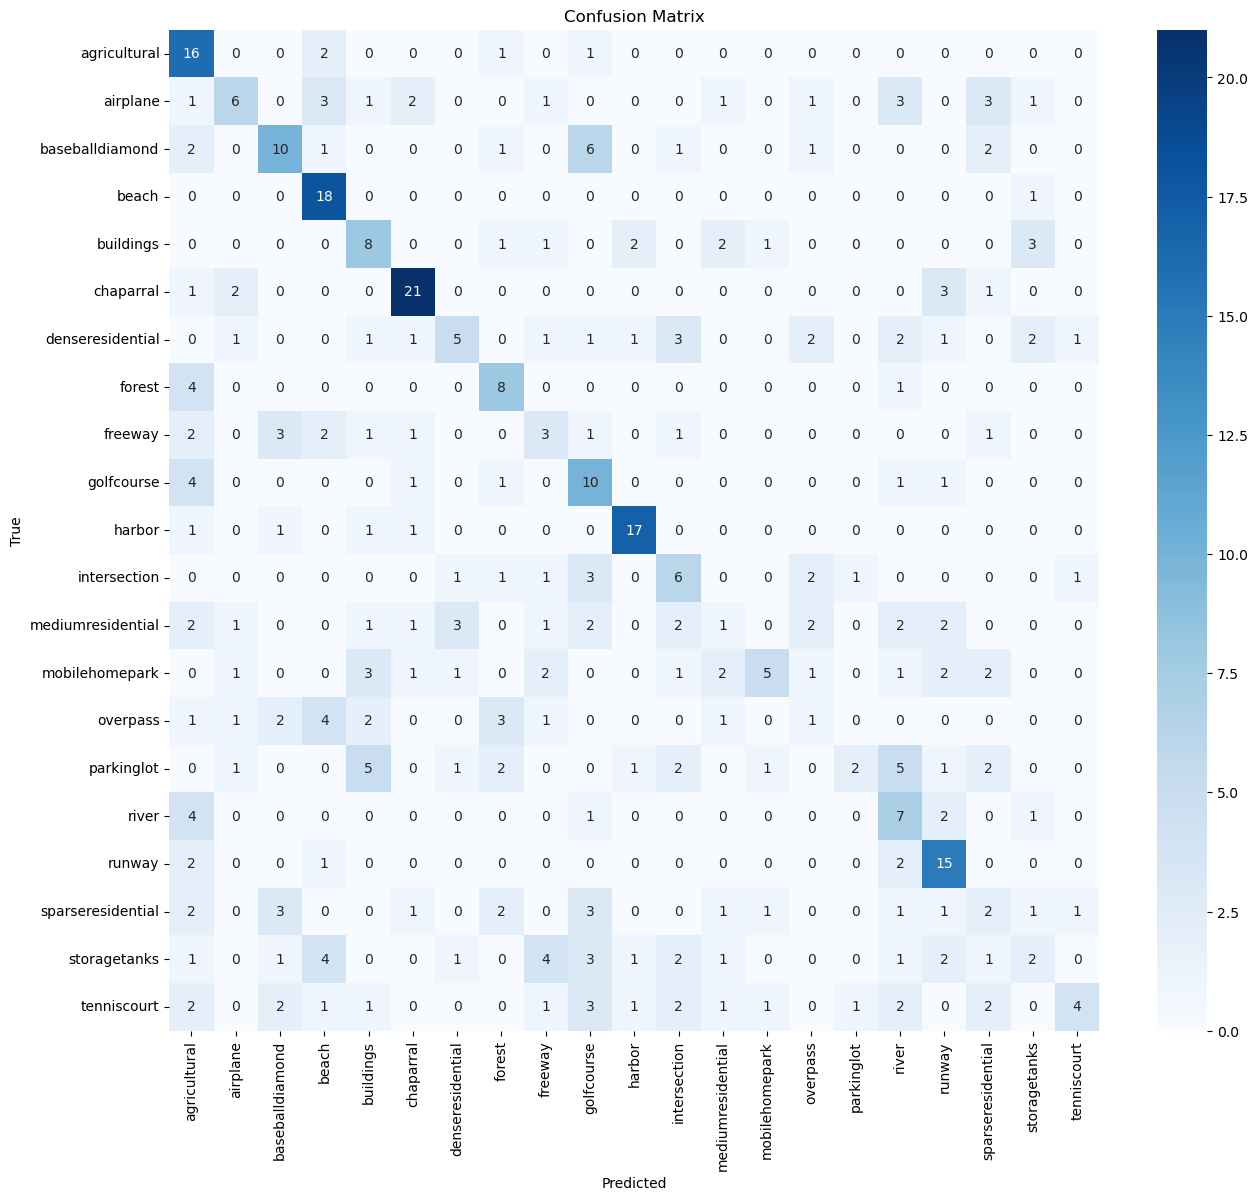
\includegraphics[width=0.5\textwidth]{Figures/methods/confusion_matrix.pdf}
    \caption[Concept of Confusion Matrices]{Conceptual representation of a confusion matrix, depicting the relationship between the predicted values and labels (actual values), adapted from \autocite{Fawcett2006}.}
    \label{fig:conf_matrix}
\end{figure}

%%%%%%%%%%
\subsubsection*{\glsentrylong{oa}}

\gls{oa} measures the proportion of correctly classified predictions out of the total predictions. It is a general measure of how well a classifier performs across all classes \autocite{Moharram.Sundaram2023,Zhao.Tu.ea2023}. It is calculated by dividing the sum of the \gls{tp} and \gls{tn} predictions by the sum of all predictions. The formula for \gls{oa}, used by the \emph{TorchMetrics} package \autocite{Torchmetrics2024a}, is described as
\begin{equation}
    \text{\gls{oa}} = \frac{1}{n}\sum_{i=1}^n 1(y_i = \hat{y}_i),
\end{equation}
whereas \( n \) is the total number of samples, \( y_i \) is the true label for the \( i \)-th sample, \( \hat{y}_i \) is the predicted label for the \( i \)-th sample, and \( 1(y_i = \hat{y}_i) \) is an indicator function that equals one if \( y_i = \hat{y}_i \), so when the prediction is correct, otherwise results to zero.

An alternative depiction of this formula including the aforementioned terms, seen in according literature like in \textcite{Tzepkenlis.Marthoglou.ea2023,Zhao.Tu.ea2023}, is
\begin{equation}
    \text{\gls{oa}} = \frac{\gls{tp} + \gls{tn}}{\gls{tp} + \gls{tn} + \gls{fp}+ \gls{fn}}.
\end{equation}

\gls{oa} should be used with caution, especially when the classes are highly imbalanced, because it can be misleading in such cases. For example, it can increase in cases where the accuracy of a class increases more than it decreases of another class \autocite{Chicco.Jurman2020,Powers.Ailab2011}. By solely looking at the \gls{oa}, this imbalanced behavior cannot be detected, which is why additional metrics are needed to evaluate the model's performance more accurately.

%%%%%%%%%%
\subsubsection*{\glsentrylong{ca}}

Because of the limitations of \gls{oa}, \gls{ca} is used as an additional metric to split the \gls{oa} into each class. It measures the proportion of correctly classified predictions for them \autocite{Fawcett2006}. A confusion matrix, as shown above, shows the class-wise accuracy, but for multiple model runs, averaging these values is done by using the arithmetic mean
\begin{equation}
    \text{\gls{ca}} = \sum_{i=1}^n \frac{\gls{tp}_i}{n},
\end{equation}
whereas \( n \) is the total number of model runs and \( \gls{tp}_i \) the \gls{tp} for the \( i \)-th sample/model run.

By looking at specific classes, conclusions about the used \gls{osm} filters can be drawn in addition to possible issues with the input data. For example, if the model has a high accuracy for the class \emph{built-up}, but a low accuracy for the class \emph{grass}, it can be assumed that the \gls{osm} filter for \emph{grass} contains contradictory \gls{osm} tags or that the input data is not sufficient for the model to extract all the information needed to correctly predict the class. The \gls{ca}, therefore, is more accurate for evaluating the accuracy of imbalanced datasets than the \gls{oa}. 

%%%%%%%%%%
\subsubsection*{\( F_{1} \) Score}

Another common performance evaluation metric is the \( F_{1} \) score. It is the harmonic mean of precision and recall, two metrics to measure the proportion of \glspl{tp} in relation to the sum of certain types of predictions. Precision measures the exactness of a model, so how many of the \glspl{tp} are actually \gls{tp}. On the other hand, recall measures the model's completeness, so how many of all as positive predicted classes were correctly predicted \autocite{Hu.Li.ea2020,Mi.Chen2020,Mohammed.Kora2023,Zhao.Tu.ea2023}. The \( F_{1} \) score is calculated by dividing the product of precision and recall by the sum of precision and recall. A high \( F_{1} \) score near one indicates a good precision and recall, and a low value towards zero indicates the opposite. Basically, the \( F_{1} \) score measures the model's accuracy, but differently than \gls{oa}, for it takes into account how the data is distributed, therefore suitable for imbalanced data \autocite{Chicco.Jurman2020,Mi.Chen2020,Powers.Ailab2011,Zhao.Tu.ea2023}.

It should be reported alongside the \gls{oa} to get a better understanding of the model's performance. This approach enhances the evaluation of both balanced and imbalanced data. Unfortunately, by using the \enquote{multiclass} parameter in the \emph{TorchMetrics} package, the result is exactly the same as \gls{oa}. Regarding these both, this results in ignoring the \( F_{1} \) score and only using the \gls{oa} for the results report.

%%%%%%%%%%
\subsubsection*{\glsentrylong{iou}}

The \gls{iou}, or as it is also sometimes called, the Jaccard Index or Jaccard Similarity Coefficient, is a metric that measures the overlap between the predicted output and the ground truth, divided by the combined area of both \autocite{Csurka.Larlus2013,Demir.Musaoglu2023}. It is defined as
\begin{equation}
    J(A,B) = \frac{|A\cap B|}{|A\cup B|} = \frac{\gls{tp}}{\gls{tp} + \gls{fp} + \gls{fn}} = \text{\gls{iou}},
\end{equation}
whereas \( A \) is the predicted output and \( B \) the ground truth \autocite{Demir.Musaoglu2023,Torchmetrics2024b}.

Using the \enquote{multiclass} parameter, this metric is applied to each class separately and then averaged to get the overall \gls{iou} value. That is why this actually is the mean \gls{iou}, as showed in \textcite{Minaee.Boykov.ea2022,Zhao.Tu.ea2023}. The (mean) \gls{iou} value lies between 0 (no overlap between predicted value and label) and 1 (perfect overlap between predicted value and label). It functions as an alternative measurement of the accuracy and is particularly useful when the location of the prediction matters, for it compares segmentation patches with each other and not only classification values \autocite{Chicco.Jurman2020,Mi.Chen2020}.

%%%%%%%%%%
\subsubsection*{Loss \& Accuracy Progression}

Finally, the loss progression in comparison to the accuracy progression can also be used as a performance metric. As explained in section \ref{subsec:loss}, the loss function is used to optimize the model's parameters during training, so the loss should decrease over time, while the accuracy should increase. Monitoring these for the training and validation sets, the models can be checked for their fitting behavior, and, therefore, the reliability of the other metrics and the overall training process.

%%%%%%%%%%
\subsection{Resource Consumption \& Efficiency}

A model can be using a lot of resources, having a high resource consumption, but still be efficient in its performance when utilizing these resources effectively. This means that if a model is using a lot of resources, but also has a high performance, it can be considered efficient, although a low resource consumption paired with a high performance would be even more efficient, of course. On the other hand, a model can be using a lot of resources, but still have a low performance, which would make it inefficient. Resource consumption and efficiency of a model are important to monitor, because they can tell if a model run is successful in reducing resource consumption while still achieving high performance \autocite{Li.Jiang.ea2021,Xu.Zhou.ea2021}.

The consumption of energy, the emission of carbon, and the overall efficiency solely of the model are difficult to monitor without additional precautions and hardware. \textcite{Mehlin.Schacht.ea2023} introduce different tools for this task, but point out that these tools oftentimes provide only an estimation and have to be reported alongside the geographic region and its infrastructure. Even then, a direct comparison and evaluation, for example of the carbon emission, is still imprecise. In addition to that, the accuracy of the model should also always be included, because achieving a lower energy consumption but also a lower accuracy, for example, is not a good trade-off \autocite{Li.Jiang.ea2021,Tao.Meng.ea2022}. Furthermore, if a code-dependent tool is used, the energy consumption can vary depending on the code and the machine it is running on \autocite{Mehlin.Schacht.ea2023}. Nevertheless, there are some metrics that can be used to estimate the resource consumption and efficiency of the model, which are described below.

%%%%%%%%%%
\subsubsection*{Runtime \& Number of Epochs}

The primary metrics for assessing a model's resource consumption and efficiency are its runtime and the number of epochs required for convergence. These metrics are a reliable indication, as long as the same hardware and software settings are used \autocite{Mehlin.Schacht.ea2023}. However, as explained also in section \ref{subsec:regularization}, less epochs or a shorter runtime do not necessarily mean a more efficient model. A shorter runtime and comparable performance imply higher efficiency, while a higher number of epochs and a longer runtime imply a higher resource consumption regardless of the performance. Similarly, a low resource consumption alongside low performance are not a good trade-off and not efficient as well. The model's total runtime serves as a indicator of its overall resource consumption, as longer runtimes typically correlate with a higher energy consumption \autocite{Li.Jiang.ea2021,Xu.Zhou.ea2021}. To enhance comparability, the time needed per epoch is calculated as well, enabling a better understanding of the model's efficiency in comparison to the performance.

%%%%%%%%%%
\subsubsection*{Model Size}

As showed in \textcite{Mehlin.Schacht.ea2023,Tao.Meng.ea2022}, the model size can also be important for the resource consumption of the model. It is usually directly correlated to the complexity of the model, therefore, needed resources to train and infer \autocite{Xu.Zhou.ea2021}.

Additionally, although today a good internet connection and enough disk space are not a rarity anymore, handling and distributing models with multiple hundreds or thousands of MB can still have an indirect impact on the model's resource consumption. The framework of the \gls{lulcu} is designed to offer an online storage of the model, so the larger the model, the more space is required on the server and cloud which themselves burn a lot of energy to offer this service. By keeping the model size low, these indirect resource consumptions can be reduced. The model size is automatically measured in MB and is the space taken up by the model on the online storage.

%%%%%%%%%%
\subsubsection*{Energy Consumption}

Regarding energy consumption, the \gls{lulcu} has an energy tracker from the \emph{pyJoules} package \autocite{PowerAPI2024} implemented, which measures the consumed energy in Millijoules. But, a large drawback of the measurement is, that it is not possible to monitor the energy consumption of the model alone. The tracker measures the energy consumption of the whole machine in its current state, which includes the main parts \gls{cpu}, \gls{ram}, and \gls{gpu}, but also cooling systems and drives, all drastically influenced by running software and the unoptimized harmonization of hardware. Running a machine with as few additional programs in the background as possible helps in getting a more accurate measurement of the model's energy consumption, but it will never be the exact amount the model has consumed. \textcite{Li.Jiang.ea2021,Mehlin.Schacht.ea2023} present other tools for energy consumption measurement as well, but all have similar drawbacks and limitations.

Because additional hardware for measuring energy could not be installed on the machine and the comparability could not be given due to the setup, this measurement is disregarded and replaced with the following one.

%%%%%%%%%%
\subsubsection*{Hardware Utilization}

Measuring the energy consumption of hardware parts without hardware-near tools is much harder than measuring their utilization, therefore, this is monitored instead. The \gls{cpu}, \gls{gpu} and its memory (\gls{vram}), as well as the \gls{ram} utilization, are measured during the model run and their maxima and averages compared. The largest focus is on the \gls{gpu}, for this part is mainly used for training the model and the largest consumer on the machine, as shown above in table \ref{tab:hardwareconfig}. Additionally, because the \gls{cpu} is the second largest consumer and also highly involved in successfully training the model, it is monitored alongside the \gls{gpu}. \gls{ram} and \gls{vram} play a minor role, because there should be a linear relationship between larger feature spaces and higher memory utilization. That is why reducing the complexity of the road network, as explained in the extension sections, is important. Still, their utilization is monitored to check for memory leaks or other issues, possibly explaining other performance or efficiency issues. 

As measuring the energy consumption, the utilization of those parts can also be influenced by running software in the background. However, the monitoring is much more detailed with more tools at hand, therefore, using the same machine configuration for all the runs and minimizing background processes, the utilization should still give better tendencies on how much the model uses the hardware resources. This gives an good estimation on how difficult it is to train the model and how much computational power is needed, giving a good insight into the resource consumption of the models.

%%%%%%%%%%
\subsubsection*{Carbon Emission}

Finally, measuring the carbon emission depends on the energy source mix of the geographical location which the machine uses \autocite{Mehlin.Schacht.ea2023}. Because this is difficult to determine, the carbon emission is not measured additionally in this study. \textcite{Li.Jiang.ea2021} suggest using a \enquote{Greenness} score for evaluating the carbon emissions of the model, but this was redeemed unfeasible for the task at hand, because it consists of multiple energy measurements, which are disregarded. The presented metrics are good indicators for the efficiency and resource consumption of the different extensions to the model, therefore, carbon emissions will not be included in this assessment.
